In this section we will be exploring data that can be commonly found in the real world.
While there are infinitely many ways to present and store data, understanding common use cases will allow us to tailor
features specifically for more common formats, and will help with creating realistic simulations in our testing.

Finding every type of commonly used data is futile, so we will attempt to approach several sectors that have a heavy
concern with data, and take a high level overview of the datasets they deal with.

The purpose of this section is to find general types of data that may have to be accounted for, as a consequence, we
will be ignoring specific features of datasets, or datasets driven by events (such as economy data being affected by a
recession, or climate data being affected by global warming).
Once a complete product is produced, a next step could be to take the previously mentioned ignored features of the
analysed datasets, and create specific implementations that account for them.

This can then be used to assign metadata without requiring provided context - e.g.: If we are given unidentified
temperature data, we could suggest adding a metadata tag linking it to our knowledge of how climate temperatures are
modeled.

\subsection{Trading}

Trading is a very data focused profession, predicting trends requires careful analysis of previous data and its effect
on the market.
For this section, we'll look at some of the more common commodities that are traded, and important data sets that are
explored for them.

\subsubsection{Energy}

Energy trading focuses on commodities that generate electricity.
Predicting fluctuations in energy prices requires analysis of data that can affect supply or demand of electricity.

The first data set we will explore is weather.
Typically weather will have a direct effect on energy prices, specifically, lower temperatures cause direct increase
in prices - leading to higher prices in the winter.


\begin{figure}[H]
    \centering
    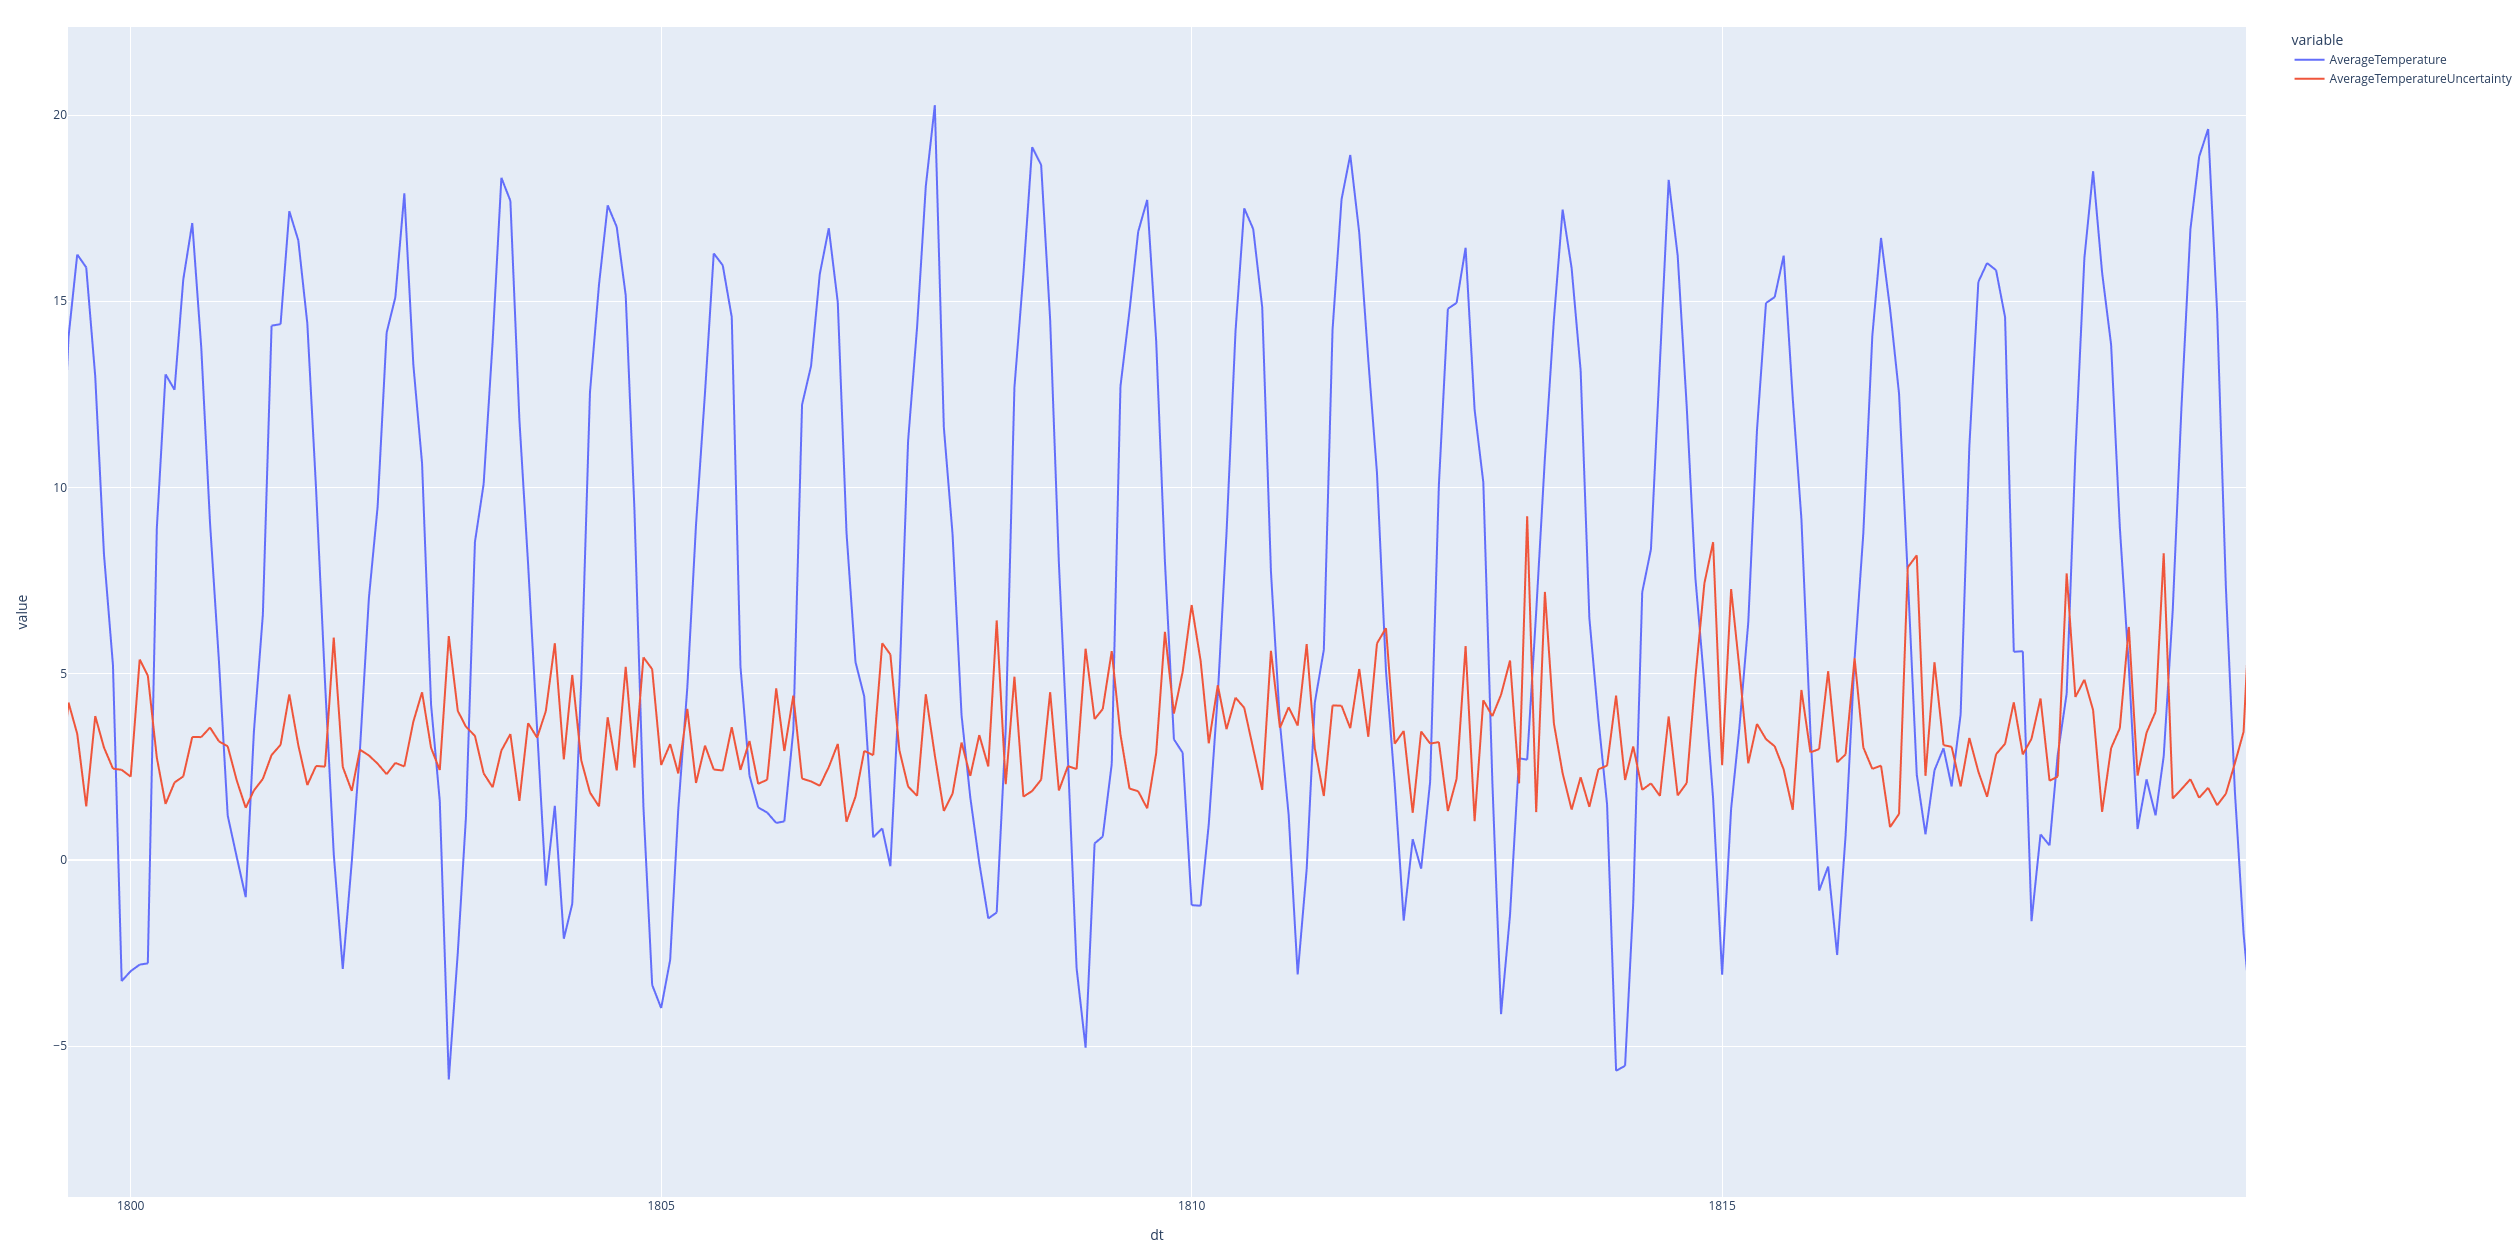
\includegraphics[width=12cm]{figures/real_data_examples/cph_average_temp}
    \caption{The average temperature in Copenhagen over a period of 20 years}
    \label{fig:real_data_climate_cph}
\end{figure}

In figure~\ref{fig:real_data_climate_cph} we plot average temperatures over 20 years - sourced from~\cite{KaggleTemperature}
we can see that temperature very reliably follows a repeating pattern that we could model as a sine wave.

\subsubsection{Currencies}

Trading currencies involves holding a currency that is predicted to increase in value relative to other currencies,
this requires analysis of data that is expected to affect the strength of a currency.

Our first focus point is inflation, as it is well understood concept with easy to model data.

\begin{figure}[H]
    \centering
    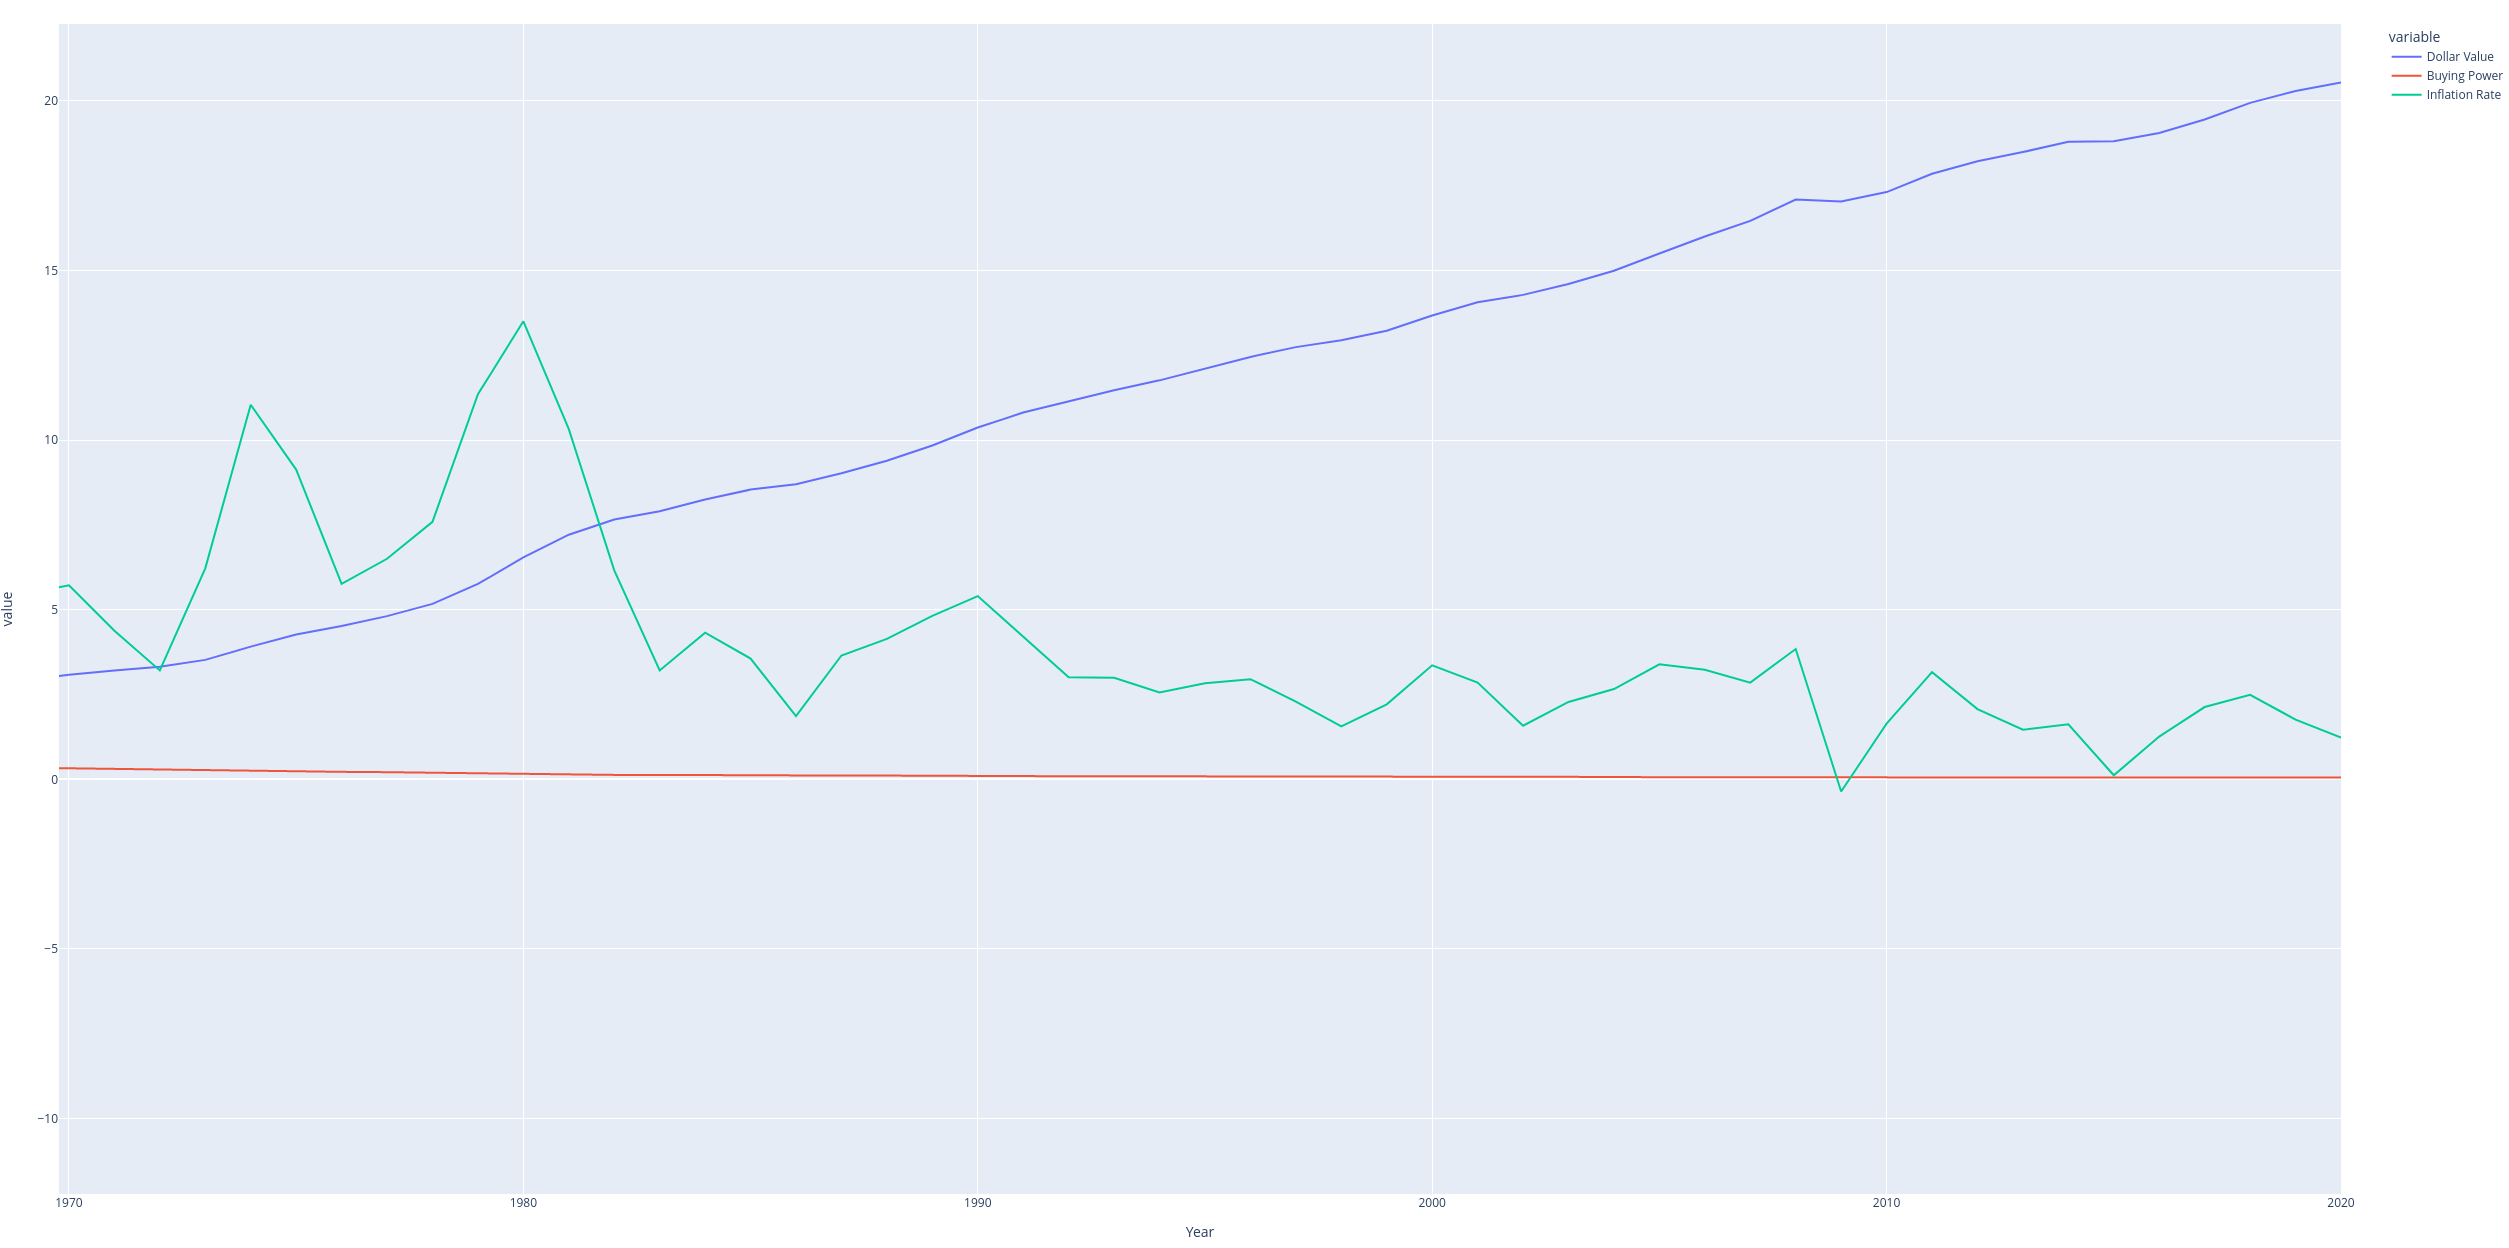
\includegraphics[width=12cm]{figures/real_data_examples/dollar_value_statistics}
    \caption{The buying power of a dollar between 1970 and 2020}
    \label{fig:real_data_inflation}
\end{figure}

In figure~\ref{fig:real_data_inflation} we plot the buying power of the dollar retrieved
from~\cite{officialdataCPIInflationUS}, which can be roughly modeled as a linear graph.
Looking at larger period ranges breaks the pattern that we've established, as specific events have led to drastic
changes before 1970, and in recent years.
It is important to remember here that our goal is not to model specific data sets, for our purposes, we will consider
these changes as simply features of this specific dataset, which may be addressed in more specialised implementations of
our software.

\subsection{E-Commerce}

Companies specialising in E-commerce use data to understand their customers needs, in-depth tracking leads to very large
dumps of various statistics, in this section we will try and identify the types of data that are considered more useful.
Naturally, companies gathering such data are unlikely to relinquish it - in an effort to bypass this setback, we have
decided to use a popular ecommerce BI solution -~\cite{GoogleAnalytics} - as a proof of concept to advertise their
product, google provides a test environment that showcases the possibilities.
For this section we will assume that the test environment contains realistic data examples.

\begin{figure}[H]
    \centering
    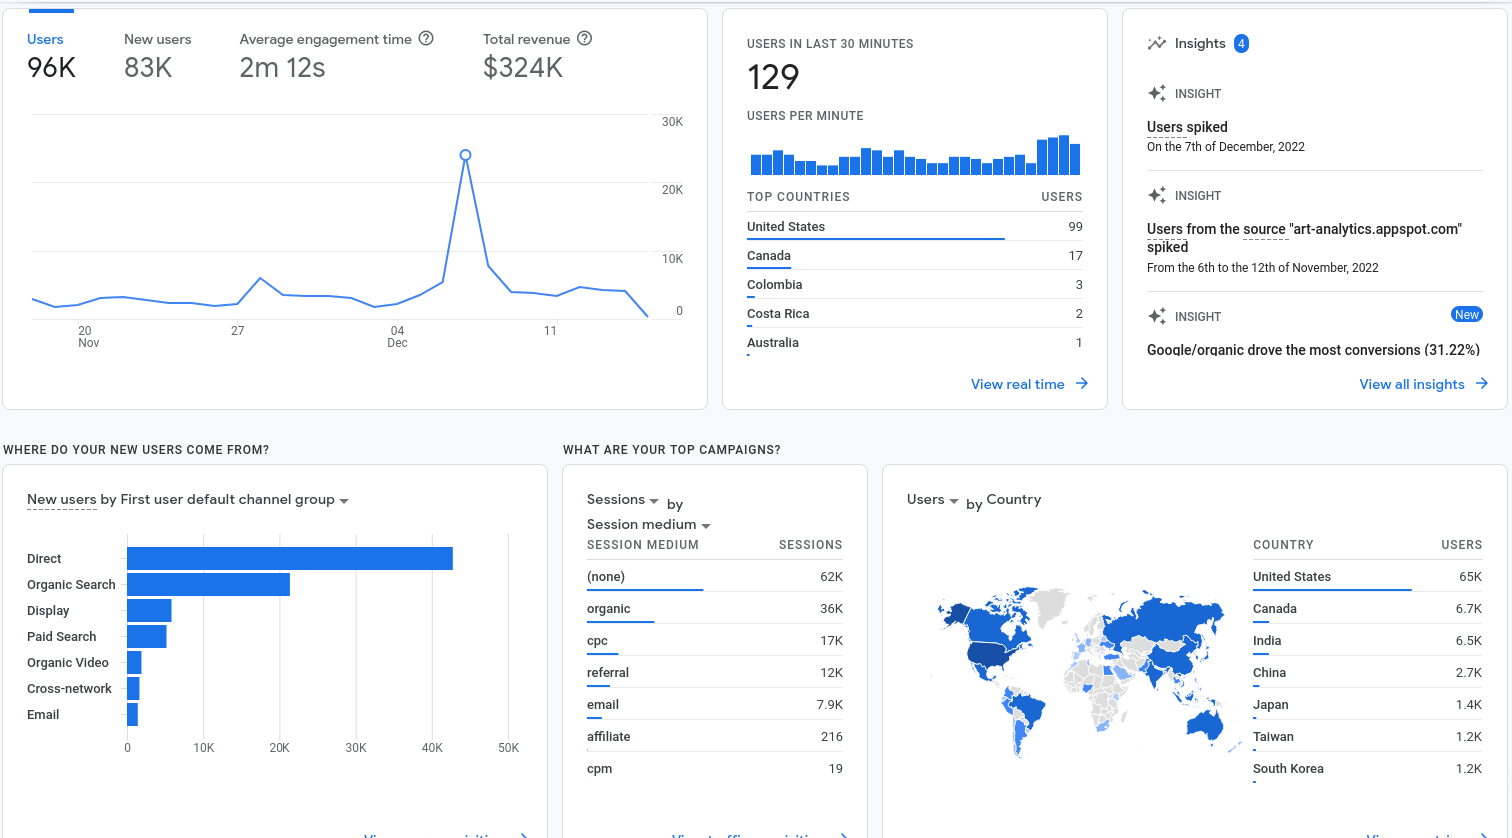
\includegraphics[width=12cm]{figures/real_data_examples/google_analytics_dashboard}
    \caption{A snapshot of a section of the google analytics dashboard showcase}
    \label{fig:google_analytics_dashboard}
\end{figure}

\begin{figure}[H]
    \centering
    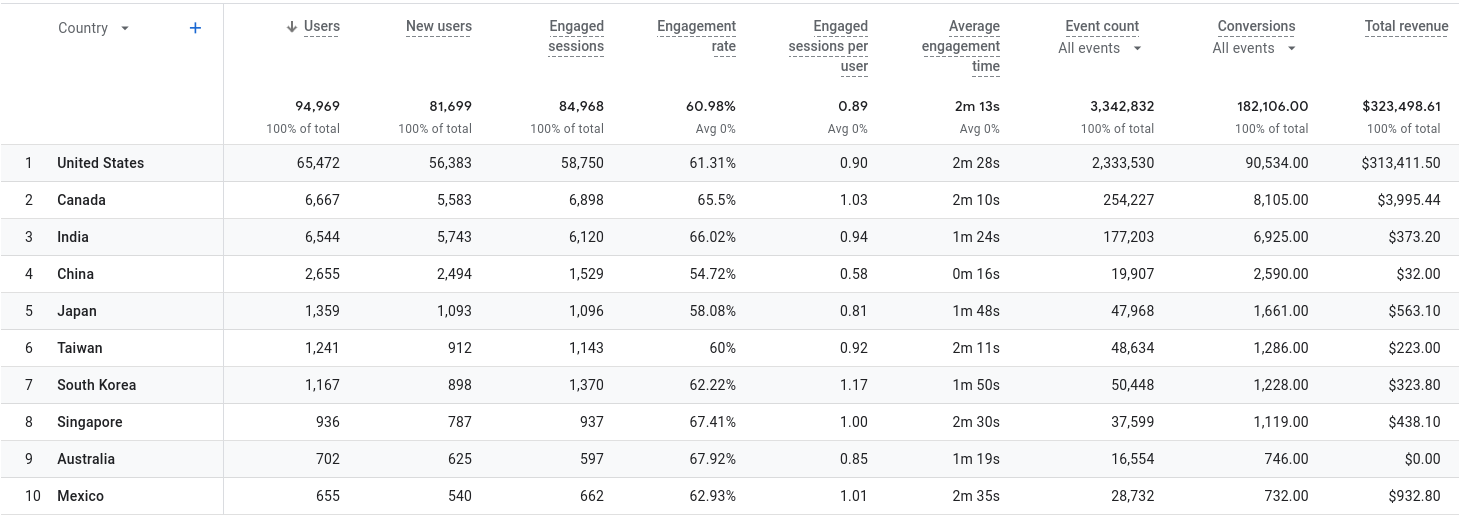
\includegraphics[width=12cm]{figures/real_data_examples/google_analytics_user_demographics}
    \caption{A snapshot of the google analytics showcase demonstrating user demographics}
    \label{fig:google_analytics_demographics}
\end{figure}

\bigbreak
The first data set we will explore is the user demographics table, as displayed in
figure~\ref{fig:google_analytics_demographics}.

While the data is largely unremarkable, it introduces a new dynamic to data entry - categorical indexes.
In previous examples, the index has been continuous, in terms of data matching this would mean that continuations of the
data set could be very simply constructed - however there is no realistic continuation of a list of countries.

The significance of such a simple fact becomes apparent when looked at in terms of data matching, as realistically we
can derive conclusions of matching data sets without exploring individual cells at all.

In practise, it will be difficult to construct algorithms that stitch together such data sets, as cells may require
specialised calculations to build, however this presents us a very simple feature to address in terms of metadata
generation.


\begin{figure}[H]
    \centering
    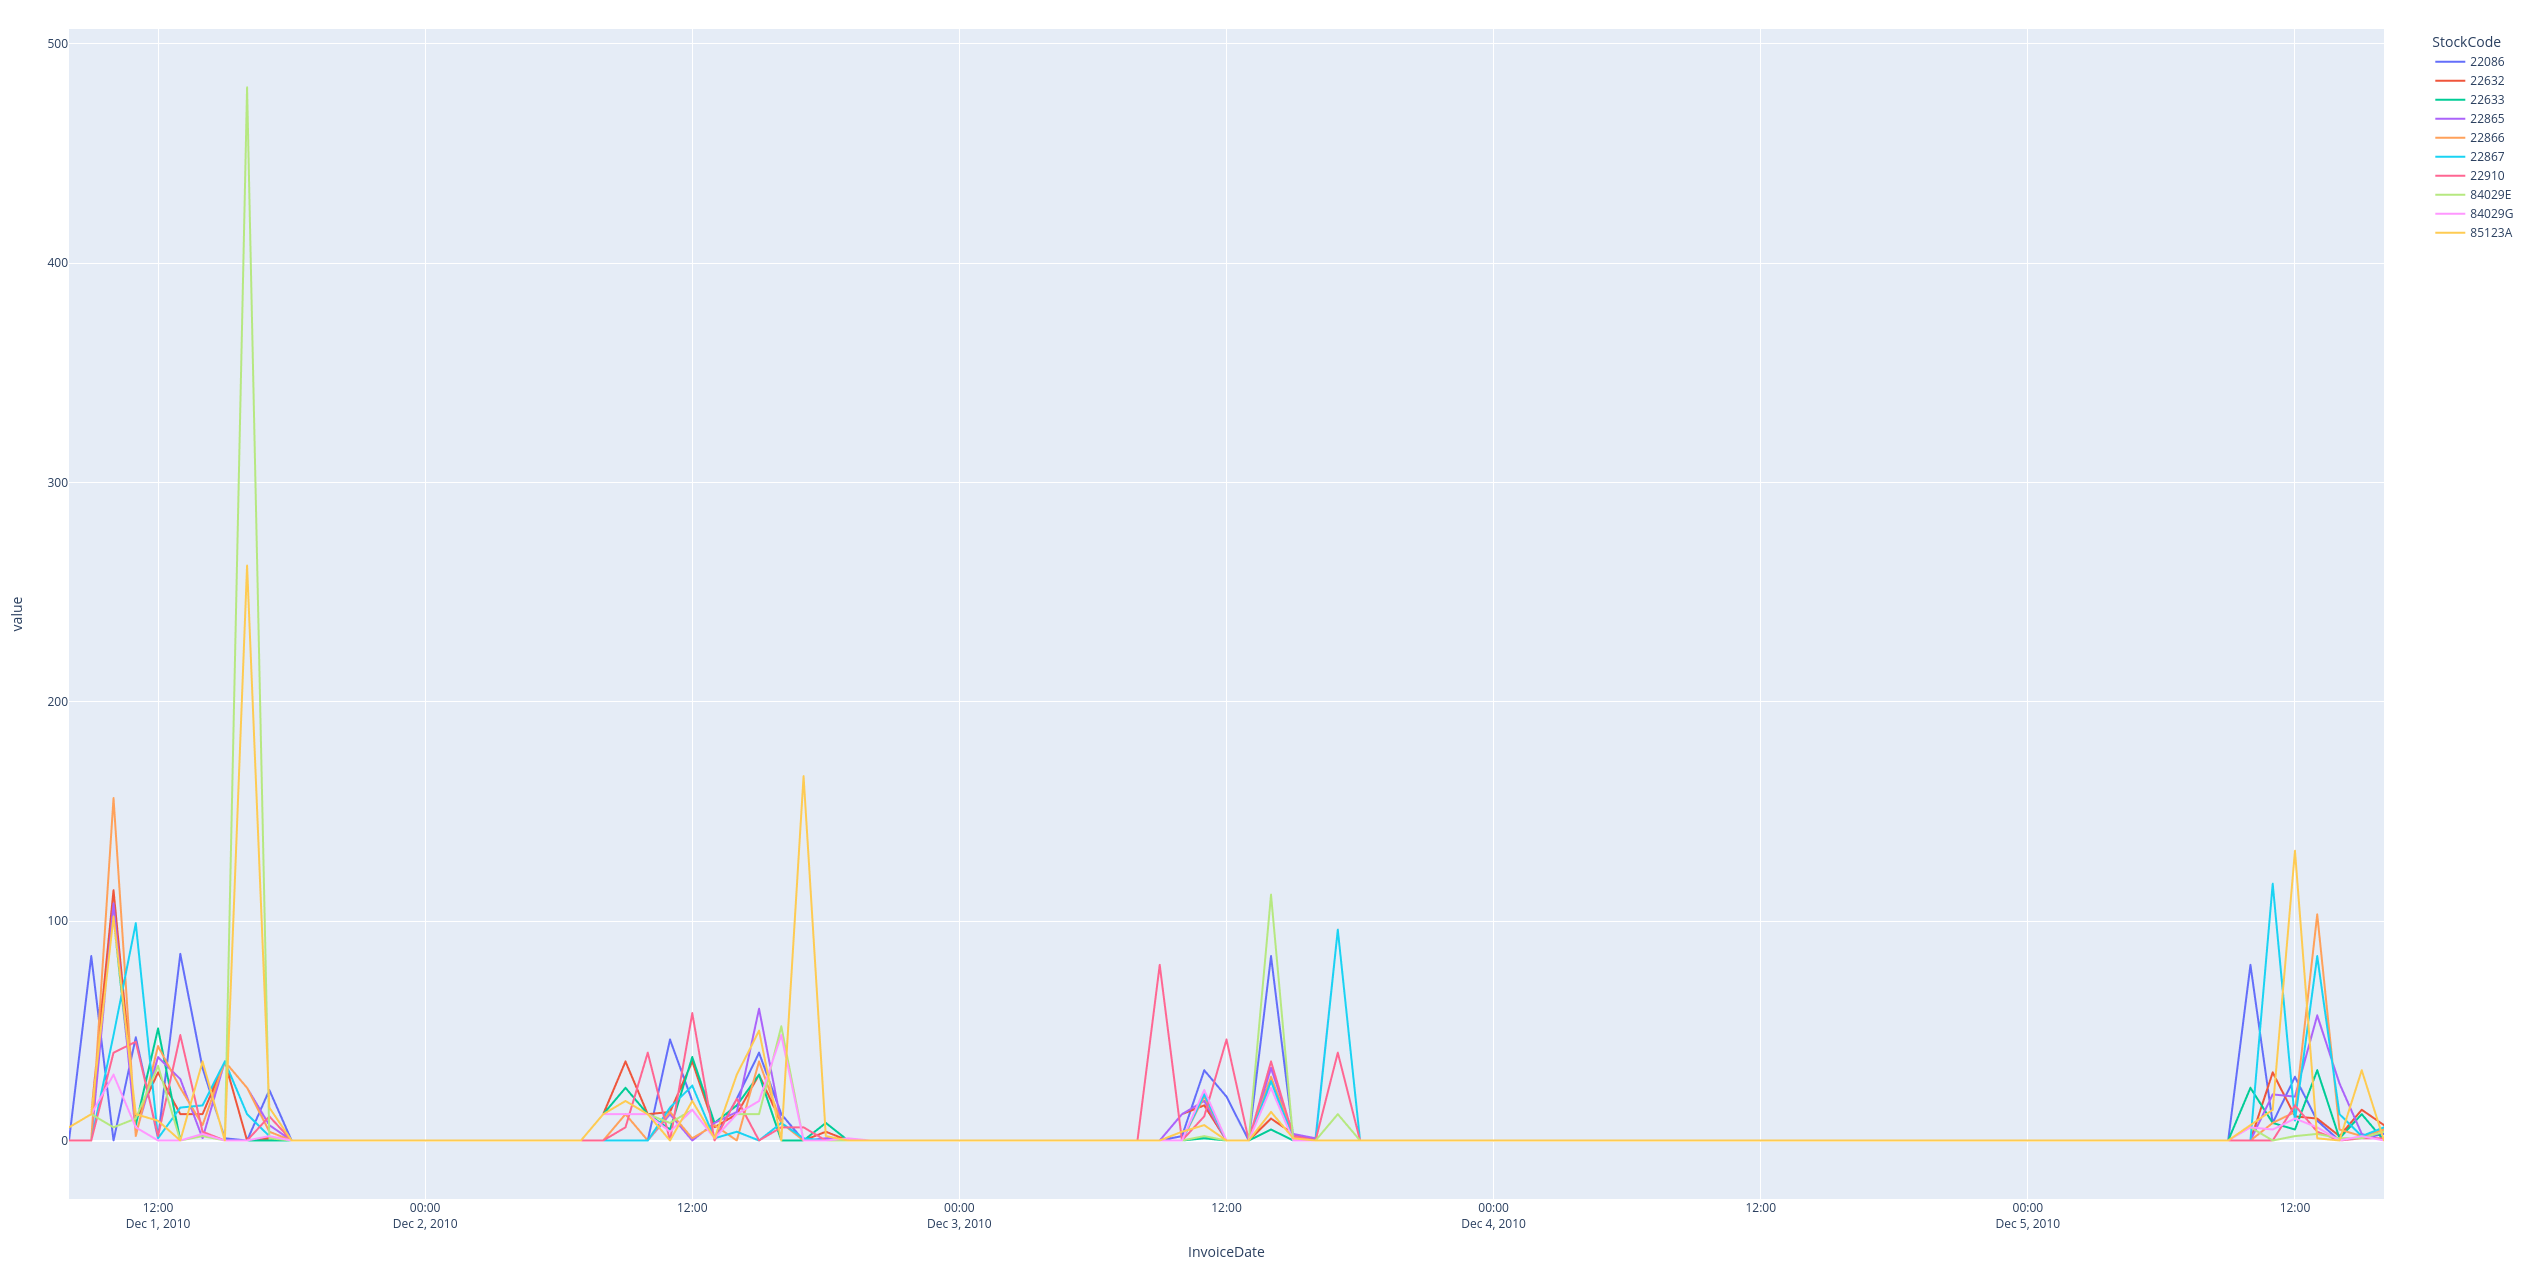
\includegraphics[width=12cm]{figures/real_data_examples/real_data_invoice_timeseries}
    \caption{A time series of quantity of invoices made for each stock code in hourly intervals}
    \label{fig:invoice_timeseries}
\end{figure}

Our next data set is a time series of invoices, retrieved from~\cite{UCIMLRepo} and with the top 20 products plotted
as hourly sums in figure~\ref{fig:invoice_timeseries}.
This data is largely unremarkable, however it has been chosen as it features a new concept to approach - here we have
our first concrete example of categorical columns.
The original data set is built by receiving an invoice event, which is then saved with various other pieces of metadata.
We can model similar datasets by creating a list of categorical data points each with a set probability of occuring.


\subsection{Medicine}

\begin{figure}[H]
    \centering
    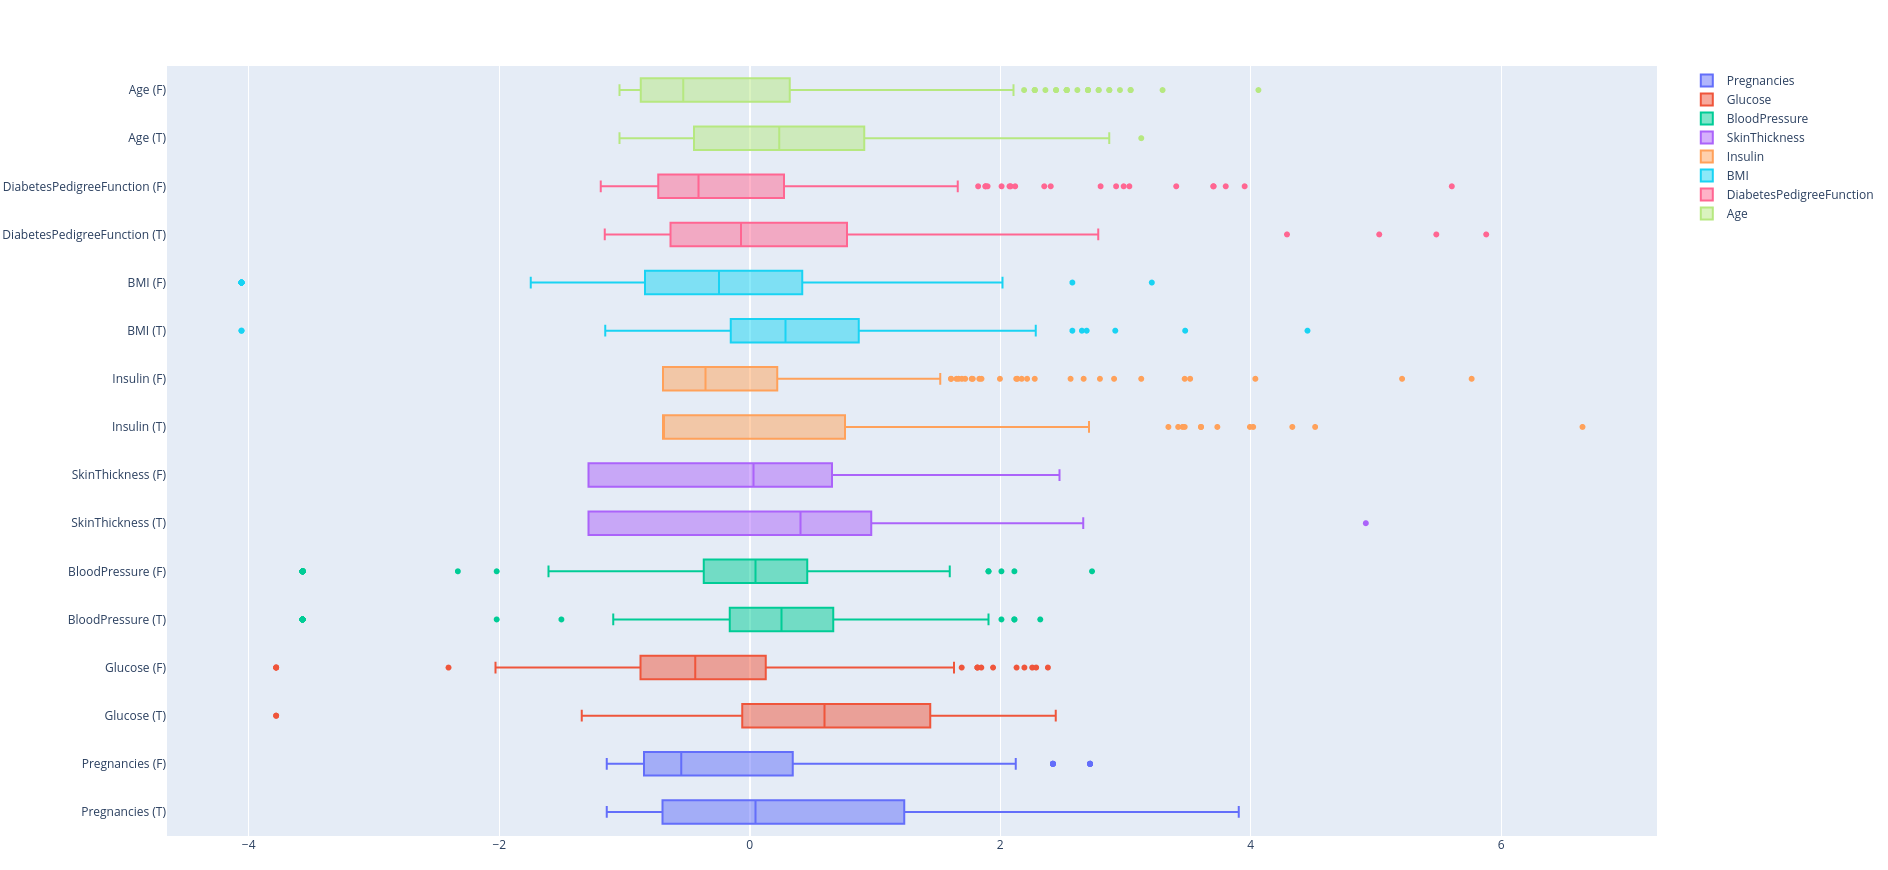
\includegraphics[width=12cm]{figures/real_data_examples/diabetes_attributes}
    \caption{A normalised representation of various attributes, compared to whether the patient has diabetes}
    \label{fig:real_data_diabetes}
\end{figure}

When looking for possible causes leading to popular conditions, a simple approach is to plot a large amount of
attributes against a large population with and without the condition.
In~\ref{fig:real_data_diabetes} we source data from~\cite{KaggleDiabetes} and plot a normalised set of values (to allow
for easier side by side comparisons) for patients without, and then with diabetes.
From a simple observation, we can easily see that values such as glucose have a strong implication on whether a patient
has diabetes.

Modelling a random data set in this fashion is already complex, as it requires building columns with a various level of
reliance on the value of other columns - however we have an additional obstacle, as the example given is already a
simplified version of this type of data.

The first additional complexity to take into account is the possibility of a categorical column having an effect on the
outcome data - as an example, a data set representing a contagious disease would likely rely on the patient's location.

Secondly, diabetes outcomes are simply true or false;
more complex or general conditions may have a range of outcomes.

Overall, we are presented with our most complex data set to match and model so far.
Our approach towards generating this type of data will be to begin by ignoring the second aforementioned complexity, as
we have decided such complex models would be out of the scope of the project, we will remain with boolean outcomes.
To approach the first complexity, we would have to create a column that has an array of columns it can be influenced by.
When influenced by a numeric column, a calculation would have to be applied to extrapolate the applied influence.
Influences of categorical data will require specific mappings of values to their respective influence.

\subsection{Reflections}

Unfortunately when attempting to research real world data, we found that open source data sets are difficult to procure.
For the purposes of simply finding data to model, we believe we have found enough varied and popular datasets to
create a usable general application, however it is very apparent that more in-depth research would be required to build
specialised metrics.


To recap, the datasets we believe are plausible and useful to model are as follows:

\textbf{Linear data}: Can be used to model anything that increases in a linear fashion in relation to counters or time.
We observed this in currency data, where inflation increases relatively linearly against time.

\textbf{Repeating wave patterns}: Can be used to model anything that maintains an alternating pattern.
We observed this in temperature data, where average temperatures remain similar during the same parts of the year.

\textbf{Fixed index data}: Can be used to model data that serves to provide an overview - continuations would not
generate extra rows.
We observed this in user demographic data, where the index consisted of the countries available in the data set.

\textbf{Categorical data}: Can be used to model data that has a set amount of values that have no continuations
of each other.
We observed similar data in e-commerce, where invoices each have a categorical stock code.

\textbf{Influenced data}: Can be used to model datasets that are influenced numerically by other columns in the data.
We observed something similar in diabetes analysis, where an outcome of 0/1 is influenced by several other values.